
%\appendix
%\makeatletter
%\renewcommand{\@chapapp}{Załącznik}
%\makeatother
%\renewcommand\thefigure{\thechapter.\arabic{figure}} 
%\renewcommand\theequation{\thechapter.\arabic{equation}} 
\renewcommand{\appendixname}{Załącznik}
\begin{appendices}

\chapter{Wybrane miary korelacji} \label{annex:correlations}
%\addcontentsline{toc}{chapter}{Załącznik A}  
%\markboth{Załącznik A}{Załącznik A}

\setcounter{figure}{0}   
\setcounter{equation}{0}   

W pracy zastosowano kilka miar statystycznych w celu zbadania współzależności zmiennych projektowych i rezultatów. Poniżej zdefiniowano użyte metody. Przedstawione informacje zaczerpnięto z prac \cite{Czaja2000,Vargha2013,Tabachnick}.

Dla problemu optymalizacji założono, że zmienne projektowe stanowią zmienne objaśniające (niezależne) wielowymiarowej zmiennej losowej, a rezultaty optymalizacji (wartości funkcji celu) stanowią zmienne objaśniane (zależne) wielowymiarowej zmiennej losowej \cite{Czaja2000}. Zależność pomiędzy zmiennymi niezależnymi i zależnymi może opisywać jeden model dla wielowymiarowej zmiennej losowej lub szereg modeli dwuwymiarowej zmiennej losowej.

\subsubsection{Współczynnik korelacji zupełnej}
Miarą wzajemnej zależności dwóch zmiennych losowych może być kowariancja między zmienną losową $\vect{X}$ i $\vect{Y}$ oznaczona jako $\mathrm{cov}(Y,X)$. Wartość kowariancji jest związana z wartościami realizacji zmiennych losowych. Sprawia to trudności w interpretacji i przy ocenie rezultatu. Kowariancja może być znormalizowana przez wartości odchylenia standardowego zmiennych losowych $\vect{X}$ i $\vect{Y}$ (oznaczonych odpowiednio jako $\sigma_X$ i $\sigma_Y$) definiując korelację (\ref{eq:annex_corr}). Wartość ta nosi nazwę współczynnika korelacji liniowej Pearsona \teng{Pearson correlation}.
\begin{equation} \label{eq:annex_corr}
	r_{xy}=\frac{\mathrm{cov}(Y,X)}{\sigma_X\cdot\sigma_Y}
\end{equation}

Dla równomiernego rozkładu prawdopodobieństwa zmiennych losowych i dla średnich wartości wszystkich $n$ próbek każdej zmiennej losowej $\vect{X}$ i $\vect{Y}$ obliczonych jako:
\begin{equation}
\mu_x=\frac{1}{n}\sum_{i=1}^{n}x_i \qquad \mu_y=\frac{1}{n}\sum_{i=1}^{n}y_i
\end{equation}
oszacowanie współczynnika korelacji liniowej określone jest następująco:
\begin{equation}
	r_{xy}=\frac{\mathrm{cov}(x,y)}{\sigma_x\cdot\sigma_y}=\frac{\sum_{i=1}^{n}(x_i-\mu_x)(y_i-\mu_y)}{\sqrt{(x_i-\mu_x)^2}\sqrt{(y_i-\mu_y)^2}}
\end{equation}
Wartość współczynnika korelacji mieści się w zakresie od -1 do 1. Im większa jest wartość bezwzględna współczynnika korelacji tym silniejsza jest liniowa zależność zmiennych losowych. Na podstawie rezultatów prób dwuwymiarowej zmiennej losowej można wykonać regresję do funkcji liniowej metodą najmniejszych kwadratów. Kwadrat współczynnika korelacji $r_{xy}^2=$ określa miarę dopasowania linii regresji do uzyskanego zbioru punków. Innymi słowy określa on stopień dokładności prognozy wartości zmiennej zależnej na podstawie znanej wartości zmiennej niezależnej i zastosowanego modelu regresji liniowej. Następujące założenia muszą być spełnione, żeby współczynnik korelacji Pearsona był miarodajny:
\begin{enumerate}
	\item realizacje zmiennej losowej $\vect{X}$ powinny być niezależne od siebie,
	\item realizacje zmiennych losowych powinny być ilościowo określone, a ich rozkład powinien być normalny,
	\item jeśli zmienna losowa $\vect{Y}$ zależy od $\vect{X}$, to zależność ta jest liniowa,
	\item realizacje zmiennej losowej $\vect{Y}$ posiadają równomierną wariancję dla zmieniającej się zmiennej $\vect{X}$ i odwrotnie.
\end{enumerate}

Pomocne w interpretacji współczynników korelacji $r$ oraz jego kwadratu $r^2$ może być zastosowanie diagramu Venna (rys. \ref{fig:venn_diag_corr}). Zmienne losowe są przedstawione na rysunku za pomocą kół. Rozmiar kół oraz ich wzajemne położenie reprezentują kilka statystycznych wielkości. Pole koła jest równe wariancji zmiennej losowej ($\sigma_X^2$ i $\sigma_Y^2$). 

\begin{figure}[hbt!]
	\centering
	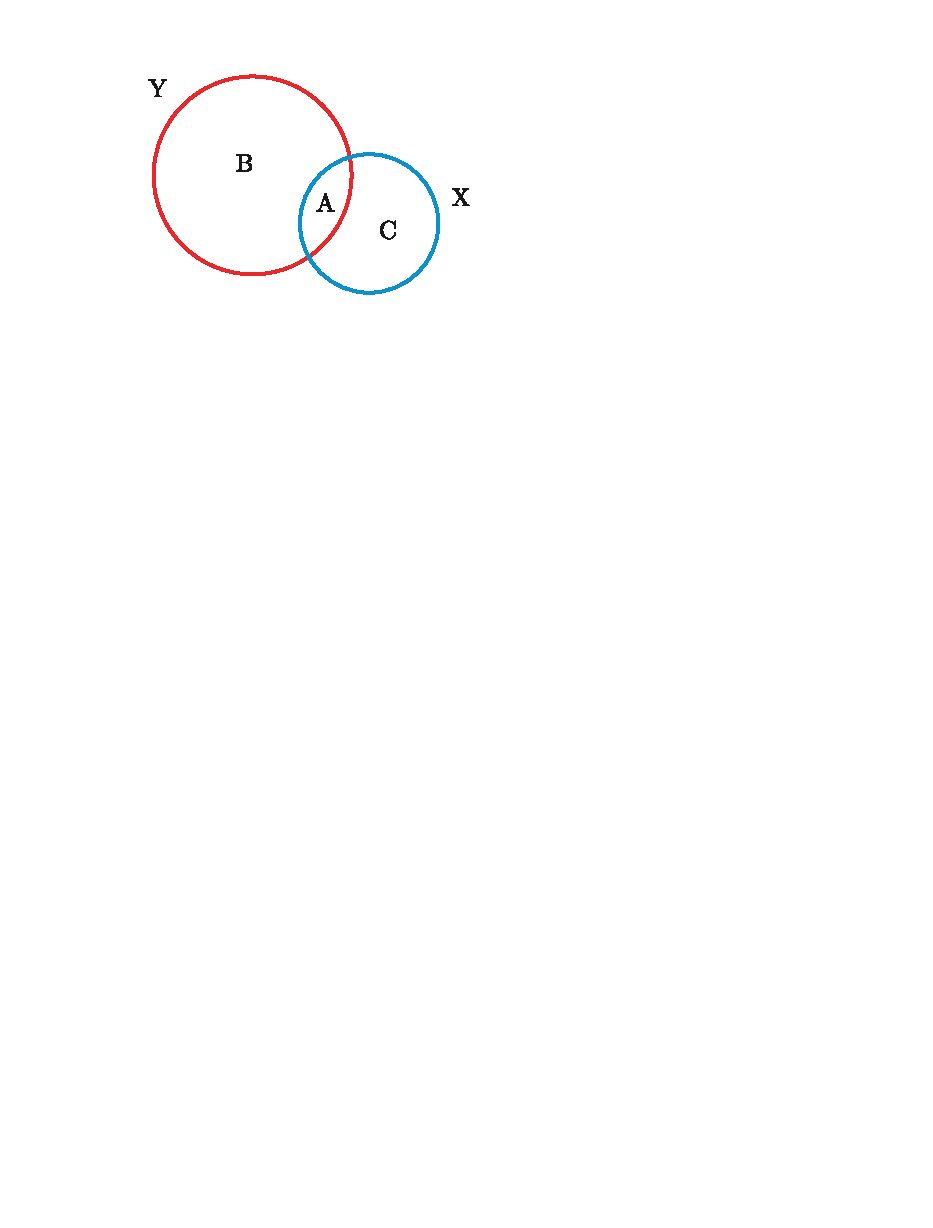
\includegraphics{WK2/korelacja/venn_diagram_corr.pdf}
	\captionsetup{justification=centering}
	\caption{Diagram Venna dla dwóch zmiennych losowych}
	\label{fig:venn_diag_corr}
\end{figure}

Jeśli występuje wpływ zmiennej niezależnej na zależną to koła częściowo nakładają się na siebie. Pole części wspólnej $A$ reprezentuje kowariancję $\mathrm{cov}(Y,X)$. Z kolei korelację oraz kwadrat korelacji można obliczyć jako:
\begin{equation}
	\begin{split}
	r_{xy} &= \frac{A}{\sqrt{A+C}\sqrt{A+B}} \\
	r_{xy}^2&= \frac{\mathrm{wariancja\;Y\;wyjaśniana\;przez\;X}}{\mathrm{całkowita\; wariancja\;Y}}=\frac{A}{A+B}
\end{split}
\end{equation}

Zwłaszcza interpretacja graficzna $r_{xy}^2$ jest pomocna. Nakładanie się okręgów prezentuje $r_{xy}^2$, a więc udział wariancji $\vect{Y}$, który może być przewidziany za pomocą $\vect{X}$. Jeżeli zmienna $\vect{X}$ w dużym stopniu wyjaśnia zmienność $\vect{Y}$ to $r_{xy}^2$ przyjmuje większą wartość, a część wspólna okręgów jest duża. Przeciwnie, kiedy korelacja $\vect{Y}$ z $\vect{X}$ jest słaba to pole wspólne jest małe. Dla zerowej korelacji okręgi są rozłączne, a dla korelacji równej 1 pokrywają się całkowicie.




\subsubsection{Współczynniki korelacji częściowej i semi-częściowej}

Kiedy istnieje więcej zmiennych losowych $\vect{X}_1, \vect{X}_2, \vect{X}_3 \dots \vect{X}_k$ to regresję liniową przeprowadza się w przestrzeni $k+1$ wymiarowej. Analogicznie do regresji z jedną zmienną niezależną (gdzie model regresji definiowany był za pomocą funkcji liniowej), w zadaniu z wieloma zmiennymi niezależnymi liniowy model regresji zdefiniowany jest jako hiperpłaszczyzna. Na przykład dla wersji z dwiema zmiennymi niezależnymi, liniowy model regresji jest płaszczyzną w przestrzeni 3D. W takim przypadku miarę wpływu jednej zmiennej niezależnej na zmienną zależną można wyrazić na różne sposoby. Pierwsza z nich określa całkowity wpływ zmiennej niezależnej na zmienną zależną i obliczana jest po prostu jako współczynnik korelacji zupełnej pomiędzy zmiennymi. Współczynniki korelacji obliczone pomiędzy wszystkimi zmiennymi losowymi często przedstawia się w postaci macierzy korelacji:
\begin{equation}
	\vect{K}=\begin{bmatrix}
1      & r_{01} &  r_{02} & \dots & r_{0k} \\
r_{10} & 1 		&  r_{12} & \dots & r_{1k} \\
r_{20} & r_{21}	&  1 	  & \dots & r_{2k} \\
\vdots & \vdots &  \vdots & \ddots & \vdots \\
r_{k0} & r_{k1} & 	r_{k2} & \dots & 1
	\end{bmatrix}
\end{equation}

Drugą ścieżką jest określenie unikalnego wpływu zmiennej niezależnej na zmienną zależną za pomocą współczynnika korelacji częściowej \teng{partial correlation} lub semi-częściowej \teng{semipartial correlation}. Określają one zależność dwóch zmiennych losowych biorąc pod uwagę wpływ innych, statystycznie zbadanych zmiennych losowych. Kiedy uwzględniany jest wpływ tylko jednej dodatkowej zmiennej, to jest to współczynnik korelacji cząstkowej pierwszego rzędu, kiedy dwóch to drugiego rzędu etc. Jak już wspomniano, współczynnik korelacji zupełnej obliczany jest dla dwóch zmiennych losowych. Jeżeli występuje więcej zmiennych losowych, to współczynnik ten nie pozwala na kontrolę pozostałych zmiennych losowych. Z tego względu określany jest również współczynnikiem korelacji zerowej. 

Niech symbol $pr_{ij\cdot 1,2,\dots,k}$ oznacz współczynnik korelacji częściowej pomiędzy zmienną losową $\vect{X}_i$ i $\vect{X}_j$, przy uwzględnieniu zmiennych $\vect{X}_1,\dots,\vect{X}_k$. Współczynnik korelacji częściowej możliwy jest do obliczenia za pomocą dopełnień algebraicznych macierzy $\vect{K}$:

\begin{equation}
		pr_{ij\cdot k} = \frac{-\mathrm{Ad}\vect{K_{ij}}}{\sqrt{\mathrm{Ad}\vect{K_{ii}}\cdot\mathrm{Ad}\vect{K_{jj}}}}
\end{equation}
gdzie: $\mathrm{Ad}\vect{K_{ij}}$ oznacza dopełnienie algebraiczne elementu $k_{ij}$ macierzy $\vect{K}$. Miarodajność współczynników korelacji częściowej wymaga spełnienia podobnych założeń jak w przypadku korelacji zupełnej.
\clearpage
Interpretację kwadratów współczynników korelacji zupełnej $r_i^2$, częściowej $pr_i^2$ i semi-częściowej $sr_i^2$ przedstawiono ponownie za pomocą diagramu Venna (rys. \ref{fig:venn_diag_part_corr}). Przyjmijmy prosty przypadek dwóch zmiennych losowych niezależnych $\vect{X}_1$, $\vect{X}_2$ i jednej zależnej $\vect{Y}$. Pola $A$ i $C$ określają w jakim stopniu wariancja zmiennej $\vect{Y}$ jest wyjaśniana przez odpowiednio zmienne $\vect{X}_1$ i $\vect{X}_2$. Pole $B$ jest częścią wariancji $Y$, która może być wytłumaczona zarówno przez $\vect{X}_1$ jak i $\vect{X}_2$.

\begin{figure}[hbt!]
	\centering
	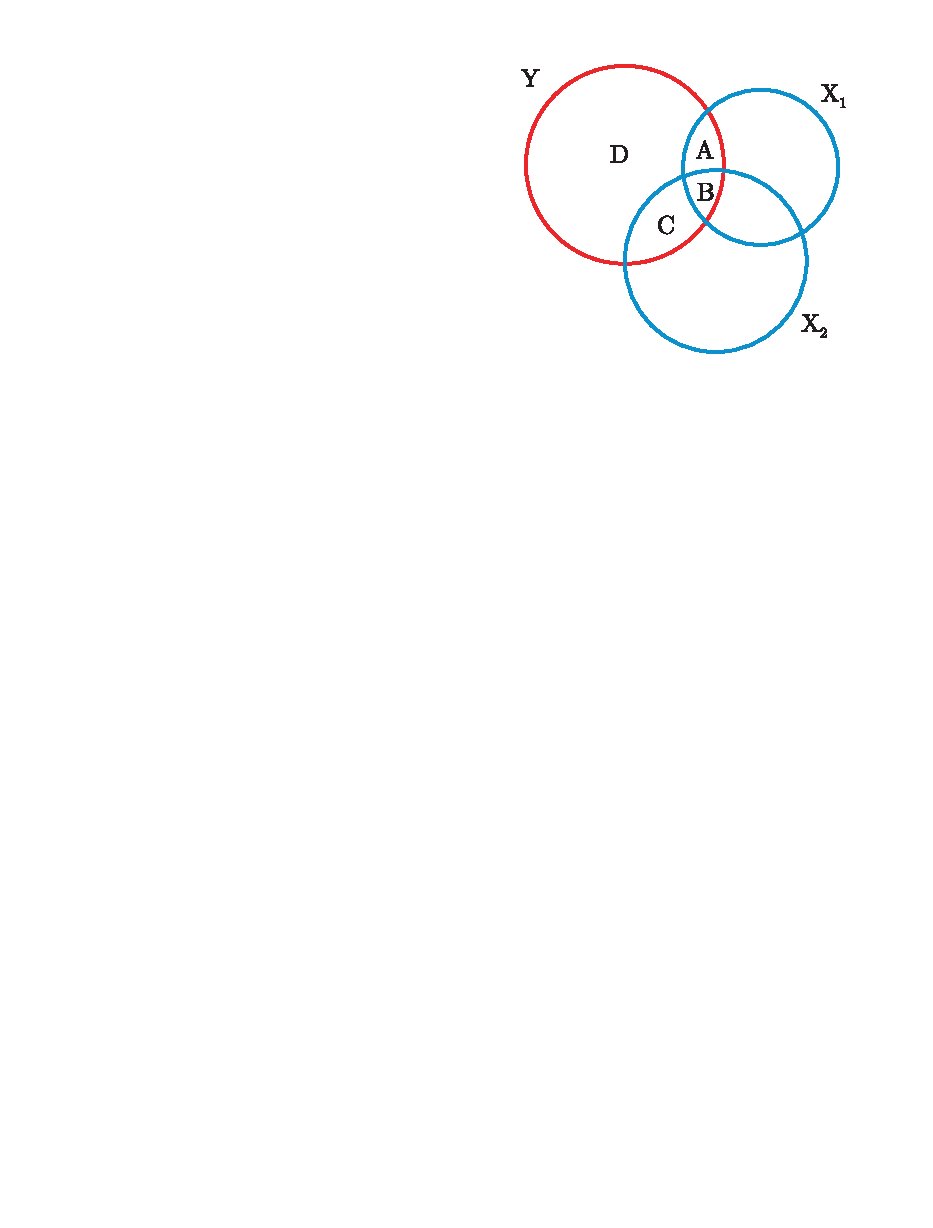
\includegraphics{WK2/korelacja/venn_diagram_part.pdf}
	\captionsetup{justification=centering}
	\caption{Diagram Venna dla trzech zmiennych losowych}
	\label{fig:venn_diag_part_corr}
\end{figure}

Korzystając z własności przedstawionego diagramu Venna, poszczególne współczynniki korelacji dla odpowiedniej zmiennej niezależnej można obliczyć następująco:
\begin{equation} \label{eqannex:zero_correlation}
	\begin{split}
		X_1:\quad& r_1^2 = \frac{A+B}{A+B+C+D} \phantom{\;\;}\\
		X_2:\quad& r_2^2 = \frac{C+B}{A+B+C+D} \\
	\end{split}
\end{equation}
\begin{equation} \label{eqannex:partial_correlation}
	\begin{split}
		X_1:\quad& pr_1^2 = \frac{A}{A+D} \phantom{\qquad\qquad}\\
		X_2:\quad& pr_2^2 = \frac{C}{C+D} \\
	\end{split}
\end{equation}
\begin{equation} \label{eqannex:semipartial_correlation}
	\begin{split}
		X_1:\quad& sr_1^2 = \frac{A}{A+B+C+D} \\
		X_2:\quad& sr_2^2 = \frac{C}{A+B+C+D} 
	\end{split}
\end{equation}

Z przedstawionej grafiki można wnioskować, że współczynnik korelacji zupełnej (\ref{eqannex:zero_correlation}) pokazuje wpływ zmiennej zależnej na całkowitą wariancję zmiennej niezależnej. Nie uwzględnia w żaden sposób istnienia wpływu innych zmiennych niezależnych. Współczynnik korelacji częściowej (\ref{eqannex:partial_correlation}) wyklucza wpływ innych zmiennych niezależnych zarówno na zmienną zależną jak i na zmienną niezależną. Z kolei współczynnik semi-korelacji (\ref{eqannex:semipartial_correlation}) wyklucza wpływ innych zmiennych niezależnych jedynie ze zmiennej niezależnej. Można więc powiedzieć, że kwadrat współczynnika semi-korelacji wyraża unikalny wkład zmiennej niezależnej na całkowitą wariancję zmiennej zależnej.






\end{appendices}